\documentclass[11pt,a4paper]{article}

\usepackage[utf8]{inputenc}
\usepackage[T1]{fontenc}
\usepackage[spanish, es-nodecimaldot]{babel}
\addto\captionsspanish{\renewcommand{\tablename}{Tabla}}
\usepackage{geometry}
\geometry{margin=2.5cm}
\usepackage{booktabs}
\usepackage{array}
\usepackage{hyperref}
\hypersetup{colorlinks=true, linkcolor=black, urlcolor=blue}
\usepackage{parskip}
\usepackage{listings}
\usepackage{xcolor}
\usepackage{graphicx}
\graphicspath{{diagrams/}}
\usepackage{float}
\usepackage{caption}
\usepackage{enumitem}

\definecolor{lightgray}{gray}{0.92}
\definecolor{codered}{RGB}{180,30,30}
\definecolor{codegreen}{RGB}{0,120,0}
\definecolor{codegray}{RGB}{100,100,100}
\definecolor{warnorange}{RGB}{200,100,0}

\lstset{
  language=Java,
  basicstyle=\ttfamily\footnotesize,
  keywordstyle=\color{blue}\bfseries,
  commentstyle=\color{codegray}\itshape,
  stringstyle=\color{codegreen},
  showstringspaces=false,
  breaklines=true,
  frame=single,
  framesep=4pt,
  xleftmargin=6pt,
  xrightmargin=6pt,
  aboveskip=6pt,
  belowskip=6pt,
  numbers=left,
  numberstyle=\tiny\color{codegray},
  numbersep=5pt,
}

\newcommand{\code}[1]{\texttt{#1}}
\newcommand{\bad}[1]{\textcolor{codered}{\textbf{#1}}}
\newcommand{\good}[1]{\textcolor{codegreen}{\textbf{#1}}}

\title{Refactorizaci\'on de la clase \code{Node}\\
       \large Extracci\'on de responsabilidades mediante el patr\'on
              \emph{Extract Class}\\[4pt]
       \normalsize \code{org.openmarkov.core} --- paquete \code{model.network}}
\author{Manuel Arias Calleja}
\date{Marzo de 2026}

\begin{document}

\maketitle
\tableofcontents
\newpage

% ===================================================================
\section{Introducci\'on}

Este documento describe la refactorizaci\'on de la clase \code{Node} del
m\'odulo \code{org.openmarkov.core}, que pas\'o de 1.037~l\'ineas a
670~l\'ineas mediante la extracci\'on de l\'ogica compleja a tres nuevas
clases de utilidad.

La refactorizaci\'on sigue el patr\'on \emph{Extract Class}
\cite{fowler2019} y se fundamenta en el \emph{Principio de
Responsabilidad \'Unica} (SRP) \cite{martin2003}.  Ambos conceptos se
explican en la secci\'on~\ref{sec:teoria} antes de describir los cambios
concretos.

% ===================================================================
\section{Fundamentos te\'oricos}
\label{sec:teoria}

\subsection{Principio de Responsabilidad \'Unica (SRP)}

El \emph{Single Responsibility Principle} establece que \textbf{una clase
debe tener una \'unica raz\'on para cambiar} \cite{martin2003}.  Si una
clase acumula m\'ultiples responsabilidades, un cambio en una de ellas
puede introducir errores en las dem\'as, porque comparten el mismo
c\'odigo fuente, los mismos campos y los mismos m\'etodos auxiliares.

\textbf{Ejemplo intuitivo:} imaginemos un cuchillo suizo que adem\'as de
cortar, destornilla, abre botellas y tiene lupa.  Si necesitamos mejorar
la hoja del cuchillo, corremos el riesgo de romper el destornillador.
En software, cada ``herramienta'' deber\'ia ser un objeto independiente.

Cuando una clase viola SRP, los s\'intomas t\'ipicos son:

\begin{itemize}
  \item La clase tiene muchas l\'ineas (cientos o miles).
  \item Los m\'etodos se agrupan en bloques tem\'aticos que no se
        relacionan entre s\'i.
  \item Los cambios en una parte de la clase obligan a re-testear partes
        no relacionadas.
  \item Es dif\'icil nombrar la clase con un sustantivo \'unico que
        describa todo lo que hace.
\end{itemize}

\subsection{Patr\'on \emph{Extract Class}}

El patr\'on \emph{Extract Class} \cite{fowler2019} es la t\'ecnica de
refactorizaci\'on que se aplica cuando una clase tiene demasiadas
responsabilidades.  Consiste en:

\begin{enumerate}
  \item Identificar un grupo cohesivo de campos y m\'etodos que forman
        una responsabilidad independiente.
  \item Crear una nueva clase con esos campos y m\'etodos.
  \item En la clase original, sustituir la l\'ogica extra\'ida por una
        delegaci\'on a la nueva clase (o eliminarla si los llamadores
        pueden usar la nueva clase directamente).
\end{enumerate}

En nuestro caso, los m\'etodos extra\'idos no usan campos privados de
\code{Node} ---solo acceden a m\'etodos p\'ublicos como
\code{getPotentials()}, \code{getParents()}, \code{getProbNet()}---,
lo que permite moverlos a \textbf{clases de utilidad est\'aticas} que
reciben el \code{Node} como par\'ametro.  Esta variante es m\'as
sencilla que la composici\'on (donde \code{Node} contendr\'ia una
referencia a la nueva clase) porque no a\~nade campos ni modifica la
construcci\'on de \code{Node}.

\subsection{Clases de utilidad est\'aticas vs. composici\'on}

Existen dos formas principales de aplicar \emph{Extract Class}:

\begin{center}
\begin{tabular}{lp{5cm}p{5cm}}
\toprule
& \textbf{Composici\'on} & \textbf{Utilidad est\'atica} \\
\midrule
Estructura &
  \code{Node} contiene un campo
  \code{NodeAbsorptionHandler handler} &
  \code{NodeAbsorptionHandler} es una clase
  con m\'etodos est\'aticos \\
\addlinespace
Llamada &
  \code{handler.absorb(variable)} &
  \code{NodeAbsorptionHandler.absorb(node, variable)} \\
\addlinespace
Ventaja &
  M\'as orientada a objetos; permite
  polimorfismo (diferentes handlers) &
  Sin estado; no modifica los constructores
  de \code{Node}; m\'as simple \\
\addlinespace
Desventaja &
  A\~nade un campo a \code{Node};
  aumenta el coste de construcci\'on &
  Menos flexible; los m\'etodos no pueden
  sobreescribirse \\
\bottomrule
\end{tabular}
\end{center}

Para esta refactorizaci\'on elegimos la variante est\'atica porque:

\begin{itemize}
  \item Los m\'etodos extra\'idos no necesitan estado propio.
  \item No se prev\'e la necesidad de m\'ultiples implementaciones
        (polimorfismo).
  \item No se modifican los constructores de \code{Node}, que es una
        clase usada en m\'as de 130~ficheros.
  \item Es coherente con el estilo del proyecto, que ya usa clases
        de utilidad est\'aticas como \code{ProbNetOperations} y
        \code{DiscretePotentialOperations}.
\end{itemize}

% ===================================================================
\section{Situaci\'on anterior: \code{Node} con 1.037 l\'ineas}
\label{sec:antes}

La clase \code{Node} acumulaba al menos seis responsabilidades distintas
en un solo fichero:

\begin{enumerate}
  \item \textbf{Identidad del nodo}: variable, tipo de nodo, red, hash,
        equals, toString.
  \item \textbf{Gesti\'on de potenciales} (CRUD): a\~nadir, eliminar,
        consultar potenciales.
  \item \textbf{Delegaci\'on al grafo}: m\'etodos de conveniencia como
        \code{getParents()}, \code{getChildren()}, \code{isParent()}.
  \item \textbf{Metadatos}: prop\'osito, relevancia, comentario,
        pol\'itica, propiedades adicionales.
  \item \textbf{Presentaci\'on visual}: coordenadas X e Y.
  \item \textbf{L\'ogica compleja de transformaci\'on}: absorci\'on de
        nodos, conversi\'on de tipos de variable, c\'alculo de funciones
        de utilidad, aplicaci\'on de restricciones de enlace.
\end{enumerate}

Las responsabilidades 1--5 son leg\'itimas para una clase que representa
un nodo en una red probabil\'istica.  La responsabilidad~6, sin embargo,
contiene \textbf{308~l\'ineas de l\'ogica de dominio compleja} que no
tiene relaci\'on con la identidad ni con el CRUD del nodo.

La figura~\ref{fig:before} muestra el diagrama UML de \code{Node} antes
de la refactorizaci\'on.

\begin{figure}[H]
\centering

\includegraphics[width=\textwidth]{before.png}
\caption{\code{Node} antes de la refactorizaci\'on.  La clase (en rojo)
         contiene m\'etodos de l\'ogica compleja que no pertenecen a la
         identidad del nodo.  Los llamadores (en amarillo) dependen
         directamente de \code{Node} para toda la funcionalidad.}
\label{fig:before}
\end{figure}

\subsection{M\'etodos problem\'aticos}

\begin{table}[H]
\centering
\small
\begin{tabular}{lrp{7cm}}
\toprule
\textbf{M\'etodo} & \textbf{L\'ineas} & \textbf{Problema} \\
\midrule
\code{absorbNodeConsistently()} & 78 &
  Multiplica/maximiza potenciales de un nodo padre sobre su hijo
  utilidad; a\~nade arcos al grafo.  L\'ogica de inferencia, no de
  identidad de nodo. \\
\code{setVariableTypeConsistently()} & 60 &
  Cambia el tipo de variable y actualiza en cascada los potenciales
  del nodo y de todos sus hijos. \\
\code{setPotentialsNodeAndChildren()} & 45 &
  M\'etodo auxiliar privado de la conversi\'on de tipos. \\
\code{resetLink()} & 17 &
  Limpia condiciones reveladas y restricciones de los arcos.
  Acoplado con la conversi\'on de tipos. \\
\code{setUniformPotential()} & 30 &
  Crea una tabla de probabilidades uniforme manualmente en lugar
  de usar \code{PotentialOperations.getUniformPotential()} que ya
  existe en el proyecto. \\
\code{getUtilityFunction()} & 28 &
  Calcula recursivamente la funci\'on de utilidad para nodos
  supervalor.  L\'ogica de inferencia. \\
\code{getApproximate*UtilityFunction()} & 50 &
  Aproxima el m\'aximo/m\'inimo de la funci\'on de utilidad.
  L\'ogica de inferencia. \\
\code{setPotentialConsistently()} & 12 &
  Asigna un potencial y aplica restricciones de enlace.
  L\'ogica de restricciones. \\
\code{samplePotentials()} & 6 &
  C\'odigo muerto: sin ning\'un llamador externo. \\
\bottomrule
\end{tabular}
\caption{M\'etodos de l\'ogica compleja en \code{Node} antes de la
         refactorizaci\'on.  Total: $\approx$326~l\'ineas.}
\label{tab:metodos-problema}
\end{table}

% ===================================================================
\section{Refactorizaci\'on realizada}
\label{sec:refactorizacion}

\subsection{Visi\'on general}

La figura~\ref{fig:srp} ilustra conceptualmente la separaci\'on de
responsabilidades aplicada.

\begin{figure}[H]
\centering
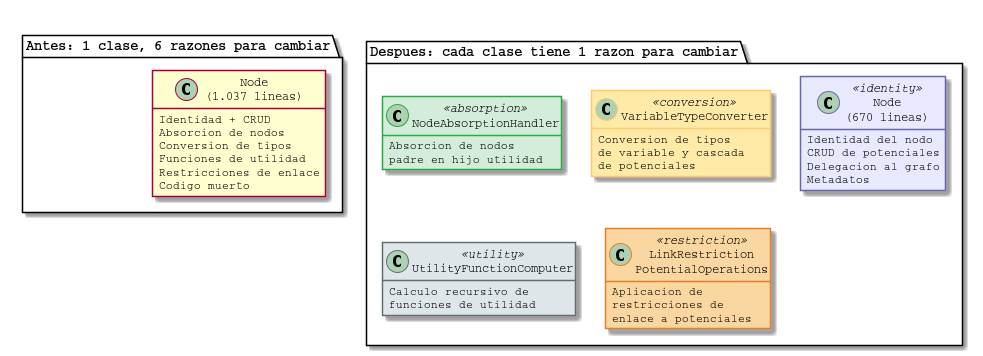
\includegraphics[width=0.9\textwidth]{srp.png}
\caption{Antes: una clase con 6~razones para cambiar.  Despu\'es: cada
         clase tiene una \'unica raz\'on para cambiar (SRP).}
\label{fig:srp}
\end{figure}

\subsection{Fase 1: Extracci\'on de \code{NodeAbsorptionHandler}}

\textbf{Responsabilidad extra\'ida:} absorci\'on de un nodo padre
(chance o decisi\'on) en su hijo utilidad.

\textbf{Antes:}
\begin{lstlisting}[caption={Llamada en \code{AbsorbNodeEdit} antes de la refactorizaci\'on}]
// AbsorbNodeEdit.doEdit()
absorbedNode.absorbNodeConsistently(absorbedVariable);
\end{lstlisting}

\textbf{Despu\'es:}
\begin{lstlisting}[caption={Llamada despu\'es de la refactorizaci\'on}]
// AbsorbNodeEdit.doEdit()
NodeAbsorptionHandler.absorbNodeConsistently(absorbedNode, absorbedVariable);
\end{lstlisting}

El m\'etodo \code{absorbNodeConsistently()} conten\'ia l\'ogica de
multiplicaci\'on y marginalizaci\'on de potenciales, creaci\'on de
\code{ExactDistrPotential}, y manipulaci\'on de arcos del grafo.
Ninguna de estas operaciones accede a campos privados de \code{Node}:
todas usan m\'etodos p\'ublicos como \code{getPotentials()},
\code{getParents()} y \code{getProbNet().addLink()}.

\textbf{\'Unico llamador:} \code{AbsorbNodeEdit.doEdit()} ---
actualizado directamente.

\subsection{Fase 2: Extracci\'on de \code{VariableTypeConverter}}

\textbf{Responsabilidad extra\'ida:} conversi\'on del tipo de variable
de un nodo y actualizaci\'on en cascada de sus potenciales y los de
sus hijos.

Se extrajeron cinco m\'etodos:
\begin{itemize}
  \item \code{setVariableTypeConsistently()} $\to$
        \code{VariableTypeConverter.convertVariableType()}
  \item \code{resetLink()} $\to$ \code{VariableTypeConverter.resetLinks()}
  \item \code{setPotentialsNodeAndChildren()} (privado, se mueve junto)
  \item \code{setUniformPotential2Node()} (se integra como m\'etodo
        privado)
  \item \code{setUniformPotential()} --- \textbf{eliminado}.  Creaba una
        tabla uniforme manualmente (30~l\'ineas) duplicando la
        funcionalidad de \code{PotentialOperations.getUniformPotential()}
        que ya exist\'ia en el proyecto.  \code{VariableTypeConverter}
        usa el m\'etodo existente.
\end{itemize}

\textbf{\'Unico llamador:} \code{VariableTypeEdit.doEdit()} ---
actualizado directamente.

\subsection{Fase 3: Extracci\'on de \code{UtilityFunctionComputer}}

\textbf{Responsabilidad extra\'ida:} c\'alculo recursivo de funciones de
utilidad para nodos supervalor (nodos con dos o m\'as padres utilidad
combinados mediante \code{SumPotential} o \code{ProductPotential}).

Se extrajeron cuatro m\'etodos:
\begin{itemize}
  \item \code{getUtilityFunction()} $\to$
        \code{UtilityFunctionComputer.computeUtilityFunction()}
  \item \code{getApproximateMaximumUtilityFunction()} $\to$
        \code{UtilityFunctionComputer.approximateMaxUtility()}
  \item \code{getApproximateMinimumUtilityFunction()} $\to$
        \code{UtilityFunctionComputer.approximateMinUtility()}
  \item \code{getApproximateMaxOrMinUtilityFunction()} (privado, se
        mueve junto)
\end{itemize}

\textbf{Qu\'e se queda en \code{Node}:} el m\'etodo
\code{isSuperValueNode()} permanece porque es una \textbf{consulta
estructural} del nodo (``\textquestiondown tiene dos o m\'as padres
utilidad?''), an\'aloga a \code{getParents()} o \code{getChildren()}.
Adem\'as, tiene 6+ llamadores en m\'odulos distintos
(\code{ProductPotential}, \code{SumPotential}, \code{TreeADDPotential},
\code{NoSuperValueNode}, \code{CEPotentialOperation},
\code{HybridElimination}).

\textbf{Llamadores migrados:}
\begin{itemize}
  \item \code{CEPotentialOperation.removeSuperValueNodes()} (m\'odulo
        \code{inference}).
  \item \code{EvidenceManager} (m\'odulo \code{gui}).
\end{itemize}

\subsection{Fase 4: Migraci\'on de \code{setPotentialConsistently()}}

El m\'etodo \code{setPotentialConsistently()} (12~l\'ineas) asignaba un
potencial al nodo y despu\'es aplicaba las restricciones de enlace si
el potencial era una \code{TablePotential} y el nodo no era de decisi\'on.

Se movi\'o a \code{LinkRestrictionPotentialOperations} (clase est\'atica
ya existente que gestiona todas las operaciones de restricci\'on de
enlace) como nuevo m\'etodo est\'atico
\code{setPotentialWithRestrictions(Node, Potential)}.

\textbf{Llamadores migrados:}
\begin{itemize}
  \item \code{SetPotentialEdit.doEdit()}, \code{undo()}, \code{redo()}
        (m\'odulo \code{core}).
  \item \code{PotentialEditDialog.setPotentialInNode()} y
        \code{removePotentialOnClose()} (m\'odulo \code{gui}).
\end{itemize}

\subsection{Fase 5: Eliminaci\'on de c\'odigo muerto}

\begin{itemize}
  \item \code{samplePotentials()} (6~l\'ineas): sin ning\'un llamador
        externo confirmado --- eliminado.
  \item C\'odigo comentado en \code{toString()}: bloques de
        \code{case COST}, \code{EFFECTIVENESS}, \code{CE} que llevaban
        comentados desde hace a\~nos --- eliminados.
  \item Todos los delegados deprecados que se introdujeron
        temporalmente durante las fases 1--4 fueron eliminados tras
        verificar que ning\'un llamador los usaba.
\end{itemize}

% ===================================================================
\section{Situaci\'on despu\'es: \code{Node} con 670 l\'ineas}
\label{sec:despues}

La figura~\ref{fig:after} muestra la arquitectura resultante.

\begin{figure}[H]
\centering

\includegraphics[width=\textwidth]{after.png}
\caption{\code{Node} despu\'es de la refactorizaci\'on.  Las clases
         nuevas (en verde) encapsulan la l\'ogica extra\'ida.  Los
         llamadores (en amarillo) usan directamente las nuevas clases.
         \code{Node} (en azul) conserva solo sus responsabilidades
         leg\'itimas.}
\label{fig:after}
\end{figure}

\subsection{Responsabilidades que permanecen en \code{Node}}

\begin{table}[H]
\centering
\small
\begin{tabular}{lrp{6.5cm}}
\toprule
\textbf{Responsabilidad} & \textbf{L\'ineas} & \textbf{Justificaci\'on} \\
\midrule
Campos + constructores + clone & 90 &
  Estado esencial del nodo. \\
Identidad (get/set variable, tipo, equals, hash, toString) & 100 &
  Contrato b\'asico de la clase. \\
CRUD de potenciales & 60 &
  Operaciones simples sobre la lista de potenciales. \\
Delegaci\'on al grafo & 80 &
  M\'etodos de conveniencia de una l\'inea:
  \code{node.getParents()} es m\'as legible que
  \code{node.getProbNet().getParents(node)}. \\
Consultas estructurales & 40 &
  \code{isSuperValueNode()}, \code{getUtilityParents()},
  \code{onlyNumericalParents()}: propiedades del nodo,
  no l\'ogica de transformaci\'on. \\
Metadatos y coordenadas & 60 &
  Getters/setters de propiedades simples.
  Las coordenadas se mantienen en \code{Node} porque son
  le\'idas/escritas por los m\'odulos \code{io} (serializaci\'on),
  \code{gui} (renderizado), \code{core} (copia) y \code{learning}. \\
\bottomrule
\end{tabular}
\caption{Responsabilidades que permanecen en \code{Node} tras la
         refactorizaci\'on.}
\label{tab:permanece}
\end{table}

% ===================================================================
\section{Ventajas del nuevo dise\~no}

\subsection{Cumplimiento del Principio de Responsabilidad \'Unica}

Cada clase tiene ahora una \'unica raz\'on para cambiar:

\begin{center}
\begin{tabular}{lp{8cm}}
\toprule
\textbf{Clase} & \textbf{Raz\'on para cambiar} \\
\midrule
\code{Node} & C\'omo se identifica y gestiona un nodo en la red \\
\code{NodeAbsorptionHandler} & C\'omo se absorbe un nodo padre en
  su hijo utilidad \\
\code{VariableTypeConverter} & C\'omo se convierte el tipo de una
  variable y se actualizan los potenciales en cascada \\
\code{UtilityFunctionComputer} & C\'omo se calcula la funci\'on de
  utilidad de un nodo supervalor \\
\bottomrule
\end{tabular}
\end{center}

\subsection{Reducci\'on de la complejidad}

\begin{center}
\begin{tabular}{lrr}
\toprule
\textbf{M\'etrica} & \textbf{Antes} & \textbf{Despu\'es} \\
\midrule
L\'ineas en \code{Node.java} & 1.037 & 670 \\
M\'etodos p\'ublicos en \code{Node} & $\approx$50 & $\approx$35 \\
Imports en \code{Node.java} & 15 & 9 \\
Dependencias de \code{Node} hacia paquete \code{potential} & 6 clases & 1 clase \\
\bottomrule
\end{tabular}
\end{center}

La reducci\'on de imports es un indicador indirecto de que \code{Node}
depende de menos conceptos.  Antes importaba \code{TablePotential},
\code{ExactDistrPotential}, \code{SumPotential},
\code{UniformPotential}, \code{PotentialRole} y
\code{DiscretePotentialOperations}.  Ahora solo importa
\code{Potential} (la interfaz base).

\subsection{Eliminaci\'on de c\'odigo duplicado}

El m\'etodo \code{setUniformPotential()} (30~l\'ineas) duplicaba la
funcionalidad de \code{PotentialOperations.getUniformPotential()} que
ya exist\'ia en el proyecto.  La nueva clase
\code{VariableTypeConverter} usa el m\'etodo existente, eliminando la
duplicaci\'on.

\subsection{Testabilidad}

Las clases extra\'idas son clases de utilidad est\'aticas sin estado.
Esto facilita enormemente su test unitario: basta crear un \code{Node}
de prueba con los potenciales adecuados y llamar al m\'etodo est\'atico.
No es necesario simular la construcci\'on completa de un \code{Node}
dentro de una \code{ProbNet} para testear la l\'ogica de absorci\'on,
conversi\'on o c\'alculo de utilidad.

\subsection{Menor riesgo de efectos secundarios}

Antes de la refactorizaci\'on, cualquier cambio en \code{Node} ---por
ejemplo, a\~nadir un nuevo tipo de potencial o cambiar el formato de
\code{toString()}--- requer\'ia revisar 1.037~l\'ineas para asegurar
que no se romp\'ia la l\'ogica de absorci\'on o de conversi\'on de
tipos.  Ahora, esa l\'ogica est\'a aislada en sus propias clases y no
se ve afectada por cambios en la identidad o presentaci\'on del nodo.

% ===================================================================
\section{Problemas que se evitan}
\label{sec:problemas}

\subsection{Problema de la clase dios (\emph{God Class})}

Una \emph{clase dios} es una clase que ``lo sabe todo y lo hace todo''.
Es un antipatr\'on reconocido \cite{riel1996} porque:

\begin{itemize}
  \item Concentra la l\'ogica en un solo punto, creando un cuello de
        botella para el desarrollo: varios desarrolladores necesitan
        modificar el mismo fichero simult\'aneamente.
  \item Dificulta la comprensi\'on: un desarrollador nuevo necesita
        entender 1.000+ l\'ineas para modificar cualquier aspecto del
        nodo.
  \item Impide la reutilizaci\'on: la l\'ogica de absorci\'on estaba
        atada a la clase \code{Node} y no pod\'ia usarse en otro
        contexto sin depender de toda la clase.
\end{itemize}

Con la refactorizaci\'on, \code{Node} deja de ser una clase dios.
Su tama\~no pasa de 1.037 a 670~l\'ineas, y la l\'ogica compleja
se distribuye en clases especializadas.

\subsection{Problema del acoplamiento indirecto}

Antes, clases como \code{AbsorbNodeEdit}, \code{VariableTypeEdit} y
\code{SetPotentialEdit} depend\'ian de \code{Node} para funcionalidad
de inferencia (multiplicaci\'on de potenciales), conversi\'on de tipos
y restricciones de enlace.  Esto significaba que un cambio en c\'omo
\code{Node} gestiona sus potenciales pod\'ia romper la l\'ogica de
absorci\'on, aunque ambas cosas no tuvieran relaci\'on.

Ahora, cada clase de edici\'on depende de la clase de utilidad espec\'ifica
que necesita.  Si cambia la l\'ogica de absorci\'on, solo se modifica
\code{NodeAbsorptionHandler}; \code{Node} y las dem\'as ediciones no se
ven afectadas.

\subsection{Problema de las dependencias excesivas}

Antes, \code{Node.java} importaba 15~clases, incluyendo
\code{DiscretePotentialOperations}, \code{TablePotential},
\code{ExactDistrPotential}, \code{SumPotential},
\code{UniformPotential}, \code{PotentialRole} y
\code{LinkRestrictionPotentialOperations}.

Estas dependencias significaban que cualquier cambio en el sistema de
potenciales (como la refactorizaci\'on de \code{TablePotential} descrita
en el documento anterior) pod\'ia requerir cambios en \code{Node},
aunque los cambios fueran irrelevantes para la identidad del nodo.

Ahora \code{Node} solo importa \code{Potential} (la interfaz base) y
las clases extra\'idas absorben las dependencias espec\'ificas que
necesitan.

% ===================================================================
\section{Verificaci\'on}

\subsection{Tests autom\'aticos}

Tras cada fase se ejecutaron los 337 tests del m\'odulo \code{core} y
el build completo de los 20~m\'odulos:

\begin{center}
\begin{tabular}{lccc}
\toprule
\textbf{Fase} & \textbf{Tests core} & \textbf{Build 20 m\'odulos} &
\textbf{Tests integraci\'on} \\
\midrule
Fase 0 (baseline) & 337 OK & OK & 361 OK \\
Fase 1 (\code{NodeAbsorptionHandler}) & 337 OK & OK & --- \\
Fase 2 (\code{VariableTypeConverter}) & 337 OK & OK & --- \\
Fase 3 (\code{UtilityFunctionComputer}) & 337 OK & OK & --- \\
Fase 4 (\code{setPotentialConsistently}) & 337 OK & OK & --- \\
Fase 5 (limpieza) & 337 OK & OK & 361 OK \\
\bottomrule
\end{tabular}
\end{center}

\subsection{Correcci\'on adicional: \code{PotentialUtils.getPotentialName()}}

Durante la verificaci\'on con los tests de integraci\'on (361 tests) se
detect\'o que el m\'etodo \code{PotentialUtils.getPotentialName()} no
recorr\'ia la jerarqu\'ia de clases al buscar la anotaci\'on
\code{@PotentialType}.  Las subclases \code{UncertainTablePotential} y
\code{StrategicTablePotential} (creadas en la refactorizaci\'on anterior
de \code{TablePotential}) no ten\'ian anotaci\'on propia, y el escritor
PGMX las grababa con un nombre vac\'io.  Al releer, el lector no
encontraba el tipo y lanzaba \code{PotentialTypeNotSupported}.

La correcci\'on fue hacer que \code{getPotentialName()} recorra la
jerarqu\'ia de clases (\code{getSuperclass()}) hasta encontrar la
anotaci\'on, de modo que \code{UncertainTablePotential} hereda el
nombre \code{"Table"} de \code{TablePotential}.

% ===================================================================
\section{Resumen de ficheros afectados}

\begin{table}[H]
\centering
\small
\begin{tabular}{llc}
\toprule
\textbf{Fichero} & \textbf{Acci\'on} & \textbf{Fase} \\
\midrule
\code{model/network/Node.java} & Simplificado & 1--5 \\
\code{model/network/NodeAbsorptionHandler.java} & Creado & 1 \\
\code{model/network/VariableTypeConverter.java} & Creado & 2 \\
\code{model/network/UtilityFunctionComputer.java} & Creado & 3 \\
\midrule
\code{action/core/AbsorbNodeEdit.java} & Caller actualizado & 1 \\
\code{action/core/VariableTypeEdit.java} & Caller actualizado & 2 \\
\code{action/core/SetPotentialEdit.java} & Caller actualizado & 4 \\
\code{potential/operation/LinkRestrictionPotentialOperations.java}
  & M\'etodo a\~nadido & 4 \\
\midrule
\code{inference/.../CEPotentialOperation.java} & Caller actualizado & 5 \\
\code{gui/.../EvidenceManager.java} & Caller actualizado & 5 \\
\code{gui/.../PotentialEditDialog.java} & Caller actualizado & 4 \\
\midrule
\code{potential/plugin/PotentialUtils.java} & Bug corregido & 5 \\
\code{integrationTests/.../Tools.java} & Caller actualizado & 5 \\
\code{integrationTests/.../Classificator.java} & Caller actualizado & 5 \\
\bottomrule
\end{tabular}
\caption{Ficheros afectados por la refactorizaci\'on de \code{Node},
         organizados por fase.}
\label{tab:ficheros}
\end{table}

% ===================================================================

\begin{thebibliography}{9}
\bibitem{martin2003}
  Robert C. Martin,
  \emph{Agile Software Development: Principles, Patterns, and Practices},
  Prentice Hall, 2003.

\bibitem{fowler2019}
  Martin Fowler,
  \emph{Refactoring: Improving the Design of Existing Code},
  2.\textsuperscript{a} edici\'on, Addison-Wesley, 2019.

\bibitem{riel1996}
  Arthur J. Riel,
  \emph{Object-Oriented Design Heuristics},
  Addison-Wesley, 1996.
\end{thebibliography}

\end{document}
